

\documentclass[uplatex,twocolumn]{jsarticle}
\usepackage[top=22mm,bottom=22mm,left=20mm,right=20mm]{geometry}
\setlength{\columnsep}{15mm}
\usepackage[T1]{fontenc}
\usepackage{txfonts}
\usepackage{wrapfig}
\usepackage[expert,deluxe]{otf}
\usepackage[dvipdfmx,hiresbb]{graphicx}
\usepackage[dvipdfmx]{hyperref}
\usepackage{pxjahyper}
\usepackage{secdot}
\usepackage{subfigure}

\makeatletter
\renewcommand{\section}{\@startsection{section}{1}{\z@}{0pt}{0.4\Cvs}{\normalfont\raggedright}}
\renewcommand{\subsection}{\@startsection{subsection}{2}{\z@}{\z@}{\z@}{\normalfont}}
\renewcommand{\subsubsection}{\@startsection{subsubsection}{3}{\z@}{\z@}{\z@}{\normalfont}}
\makeatother
%ここから上を編集する必要はない.



\setlength\textfloatsep{0pt}

%タイトルと学生番号,名前だけ編集すること
\title{\vspace{-5mm}\fontsize{14pt}{0pt}\selectfont GitHubを用いた開発フローの判別分析}
\author{\normalsize プロジェクトマネジメントコース・ソフトウェア開発管理グループ 矢吹研究室 1242132 若月 純}
\date{}
\pagestyle{empty}
\begin{document}
\fontsize{10.5pt}{\baselineskip}\selectfont
\maketitle





%以下が本文
\section{研究の背景}
\makeatletter\renewcommand{\section}{\@startsection{section}{1}{\z@}{0.6\Cvs}{0.4\Cvs}{\normalfont\raggedright}}\makeatother%余白の調整(気にしなくていい)


ソフトウェア開発では,GitHubを用いることが多い.GitHubは,バージョン管理システムに加え,branch,PullRequest,Issuesといった開発を補助する機能を提供するサービスである. 
GitHubを使用する手順を開発フローと呼ぶ.現在わかっている開発フローの数は13個ある\cite{onodera2015}.開発フローの例を1つあげる.GitHub Flowは,作業をするbranchを作成し,完成したら統合する.というような開発フローである.この開発フローはとてもシンプルなため,開発フローを実施するまでの学習コストは,抑えられるが,開発規模が大きい場合,PullRequestがたまりやすく,コードレビューに時間がかかってしまうことがある\cite{okumura2013}.
このように開発フローは,メリット・デメリットがある.そのため,開発フローをプロジェクトの性質から選択する基準が必要である. 


\section{目的}
GitHubを用いたソフトウェア開発プロジェクトの性質において,適切な開発フローを選択できるようにするための基準を提供する.

\section{研究方法}
初めに,GitHub上のプロジェクトから,プロジェクトの性質と開発フローを調査する.プロジェクトの性質は,行数,ファイル数,バイト数,Watch数,Star数,Fork数,Commit数,branch数,Release数,人数,Issues数,PullRequest数,Label数,Milestone数,Wiki数である.
次に,調査したデータの分析をする.ランダムに2種類のデータに分け,決定木分析を行う.

\section{成果物のイメージ}
GitHubを用いたソフトウェア開発プロジェクトの性質において,適切な開発フローを選択できるようにするための判断基準が求められる.
\section{進捗状況}
GitHub上の32件のプロジェクトから,プロジェクトの性質と開発フローを調査し,分析を行った.
プロジェクトの性質は,行数,ファイル数,バイト数,Watch数,Star数,Fork数,Commit数,branch数,Release数,人数,Issues数,PullRequest数,Label数,Milestone数,Wiki数,言語を調査した.
開発フローは,Git Flow,GitHub Flow,LINE Flow,Stable Flow,WIP Flowの5種類だった.

32件のプロジェクトを半分にわけ,それぞれ決定木分析を行った結果が図\ref{fig:examdecisiontree}である. 
Issues数,file数,言語,行数,バイト数により,選択される開発フローが異なることがわかった.これにより,プロジェクトの規模により選択される開発フローが異なると言える.

\begin{figure}
	\subfigure[決定木]{%
		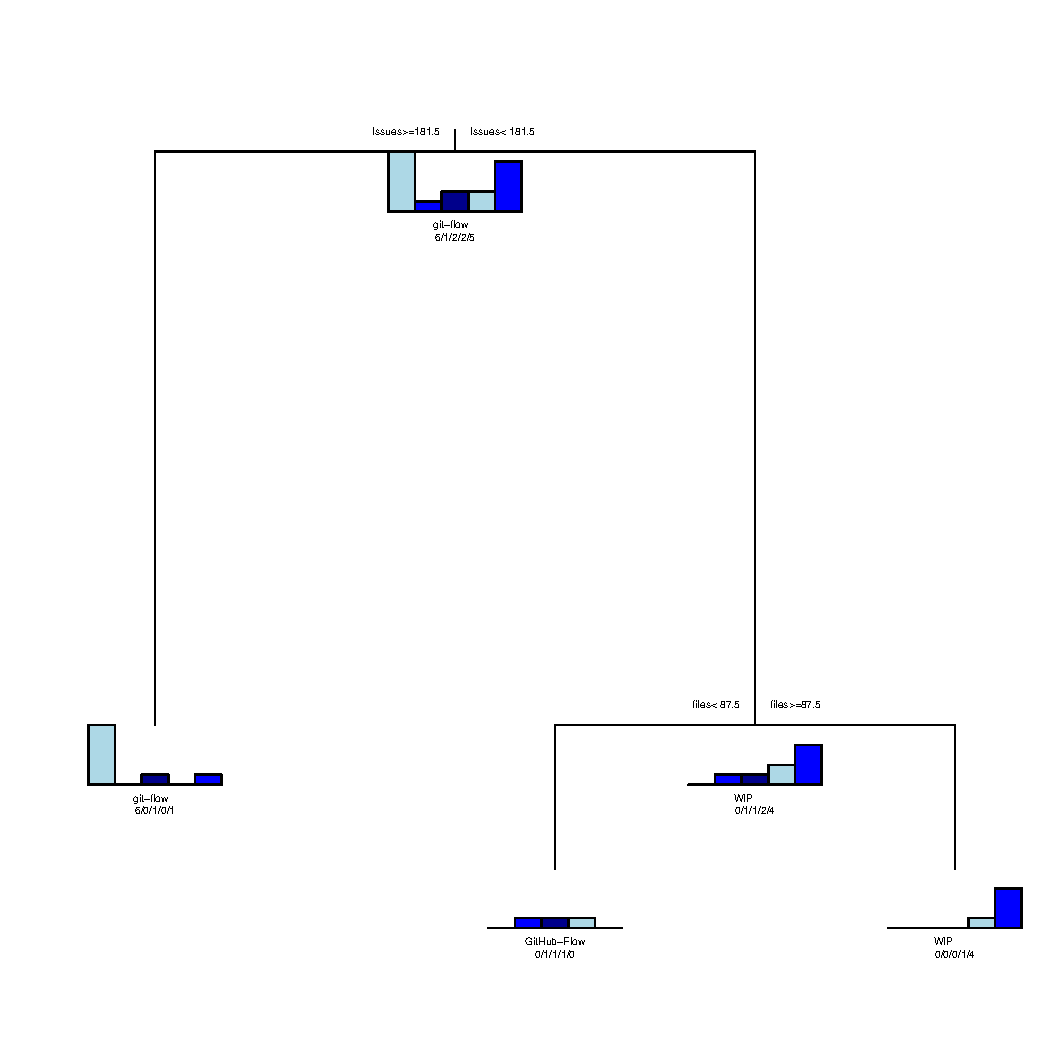
\includegraphics[clip, height=0.5\columnwidth]{1.pdf}}%
	\subfigure[決定木]{%
		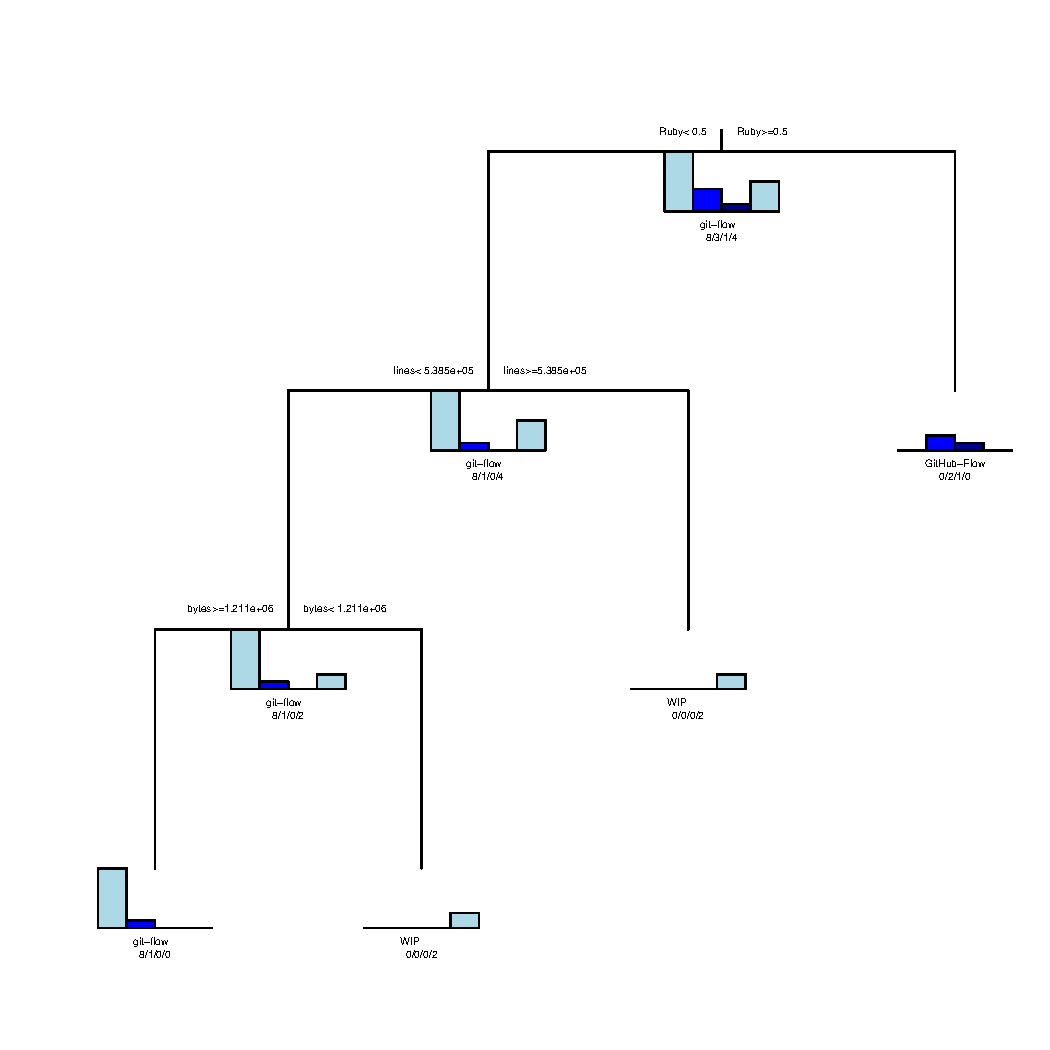
\includegraphics[clip, height=0.5\columnwidth]{2.pdf}}%
	\caption{決定木分析の結果}
	\label{fig:examdecisiontree}
\end{figure}

\section{今後の計画}

時系列データを分析に含めた場合,基準にどのような変化があるか調査する.そうすることで,大人数で開発のスピードが速い場合と少人数で開発のスピードが遅い場合では,どのような変化があるか求められる.

\bibliographystyle{junsrt}
\bibliography{biblio}%「biblio.bib」というファイルが必要.

\end{document}
